\chapter{Технологическая часть}

В данном разделе обоснован выбор средств реализации ПО, описаны формат входных данных и интерфейс пользователя и проведено функциональное тестирование.

\section{Выбор средств реализации}

В качестве языка разработки был выбран Go~\cite{go} в силу следующих причин:
\begin{itemize}
    \item в стандартной библиотеке языка присутствует поддержка всех структур данных, выбранных по результатам проектирования;
    \item средствами языка можно реализовать все алгоритмы, выбранные в результате проектирования.
\end{itemize}

\section{Формат входных данных}

Пользователю необходимо передавать ПО следующие данные:
\begin{itemize}
    \item описания объектов;
    \item информация об источниках света;
    \item информация о наблюдателе;
    \item информация о шрифте;
    \item подмножество доступных символов.
\end{itemize}

Для представления описаний объектов был выбран универсальный формат OBJ~\cite{obj} в силу того, что он позволяет передавать всю информацию, необходимую ПО для представления объекта:
\begin{itemize}
    \item список вершин;
    \item нормали к вершинам;
    \item список граней.
\end{itemize}

Информацию об источниках света пользователь указывает, вводя их координаты в пространстве и интенсивность, представленные в виде вещественных чисел.

Информацию о наблюдателе пользователь указывает, вводя его координату на оси $Z$.

Для представления информации о шрифте выбран формат TTF~\cite{ttf} в силу того, что он позволяет передавать векторные представления символов ASCII.

Доступные символы указываются пользователем в формате JSON~\cite{json} или TXT, так как оба формата позволяют передавать массивы символов.

\section{Интерфейс пользователя}

Для реализации текстового интерфейса взаимодействия была выбрана библиотека tui-go~\cite{tui}, так как:

\begin{itemize}
	\item средств библиотеки достаточно для работы с растровой графикой и вывода её в терминал;
	\item библиотека является кроссплатформенной.
\end{itemize}

Интерфейс содержит в себе окно вывода информации и поле ввода, через которое происходит взаимодействие с ПО. Пользователь управляет программой с помощью набора команд:
\begin{itemize}
    \item команда загрузки: l ПУТЬ\_К\_ФАЙЛУ;
    \item команда удаления: rm ID;
    \item команда вращения: r ID УГОЛ ОСЬ(x/y/z);
    \item команда перемещения: t ID tX tY tZ;
    \item команда масштабирования: s ID sX sY sZ;
    \item команда добавления источника света: ls X Y Z ЯРКОСТЬ;
    \item команда удаления источника света: rmls ID;
    \item команда перемещения камеры: mv РАССТОЯНИЕ;
    \item команда выхода: q.
\end{itemize}

\section{Модульное тестирование}

Модульное тестирование проводилось с помощью стандартного пакета Go -- testing. 

В качестве меры качества покрытия кода использовалась метрика стандартной утилиты cover входящей в состав Go, которая измеряет покрытие кода как процент от выполненных хотя бы единожды выражений~\cite{cover}.

Тестами были покрыты математические модули, модули матричных преобразований, отсечения и чтения объектов.

Результаты тестов с покрытием кода по модулям:

\begin{verbatim}
Running tests in internal/renderer...
ok
coverage: 29.5% of statements
Running tests in internal/object...
ok
coverage: 94.4% of statements
Running tests in internal/transformer...
ok
coverage: 36.5% of statement
\end{verbatim}

Все модульные тесты были пройдены.

\section{Функциональное тестирование}

В рамках функционального тестирования были проанализированы отдельные изображения, полученные с помощью разработанного программного обеспечения.

Для получения изображений был реализован отдельный вариант сборки, генерирующий изображения для заданных объектов с заданным освещением и сохраняющий их в виде текстовых файлов.

На рисунках \ref{fig:test1}-\ref{fig:test4} представлена модель сферы, освещенная источниками света, находящимися на различных позициях. Радиус сферы равен 5, центр совпадает с началом координат.

На рисунке \ref{fig:test1} источник света находится в точке с координатами (10, 10, -10). Сфера освещена корректно.

\begin{figure}[H]
    \centering
    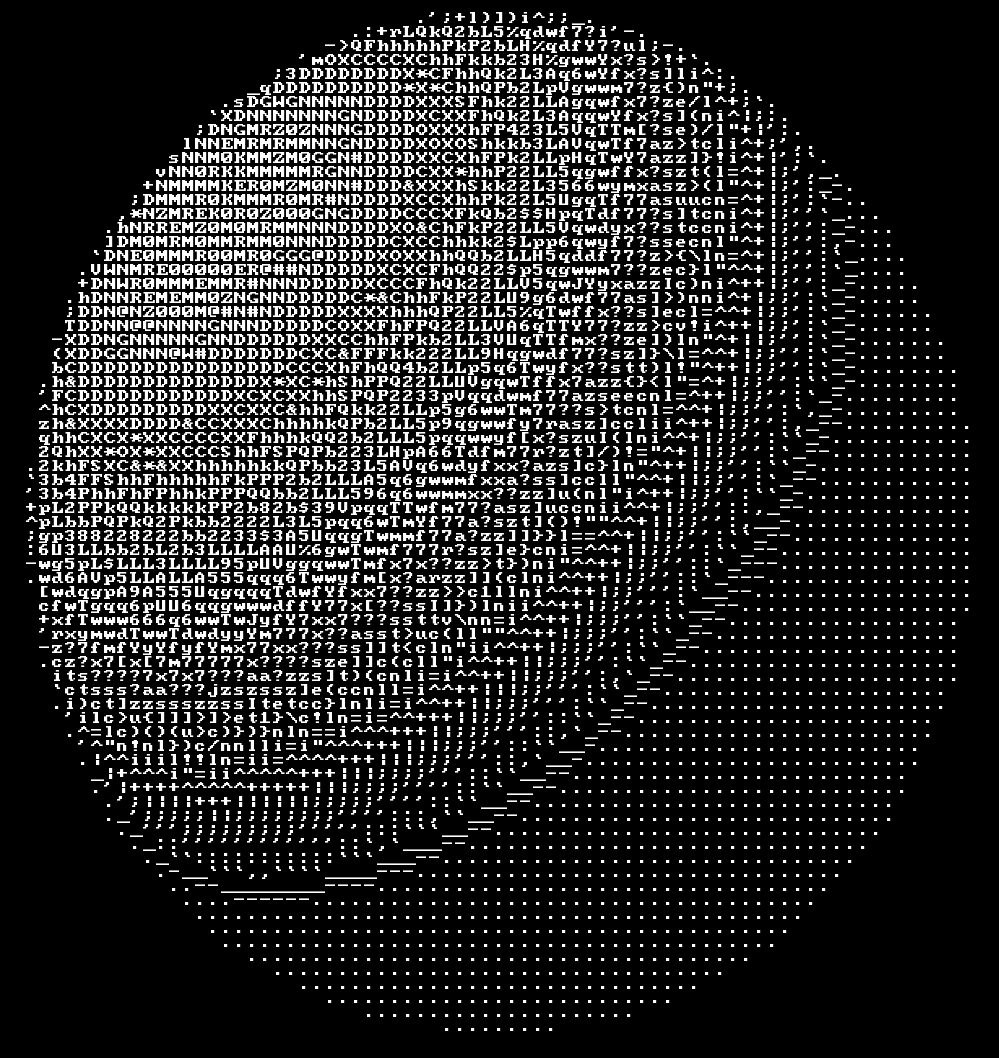
\includegraphics[scale=0.2]{images/test1.png}
    \caption{Источник света находится в точке с координатами (10, 10, -10)}
    \label{fig:test1}
\end{figure}

На рисунке \ref{fig:test2} источник света находится в точке с координатами (-10, -10, 10). Сфера освещена корректно.

\begin{figure}[H]
    \centering
    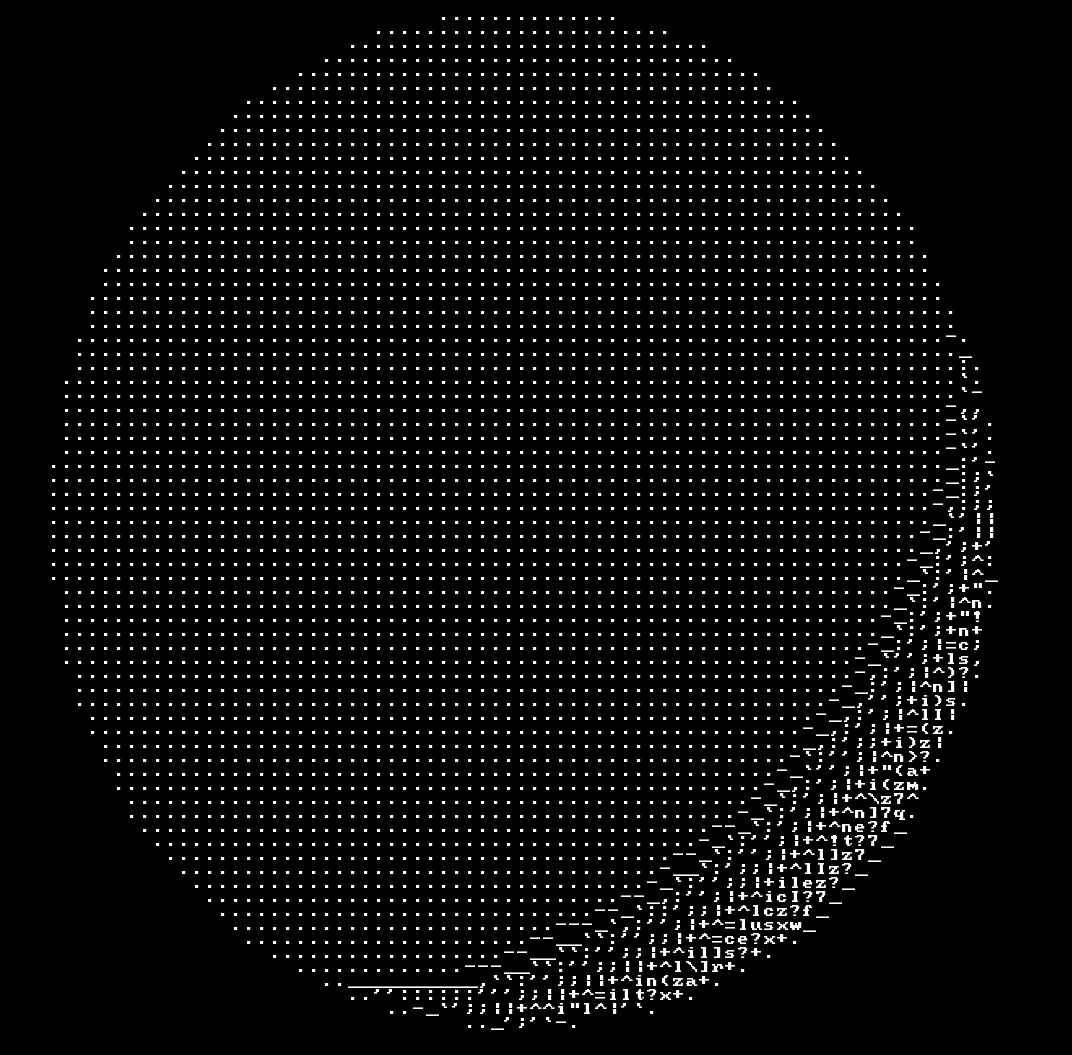
\includegraphics[scale=0.2]{images/test2.png}
    \caption{Источник света находится в точке с координатами (-10, -10, 10)}
    \label{fig:test2}
\end{figure}

На рисунке \ref{fig:test3} источник света находится в точке с координатами (0, 0, 0), то есть внутри сферы. Как и ожидалось, сфера не освещена.

\begin{figure}[H]
    \centering
    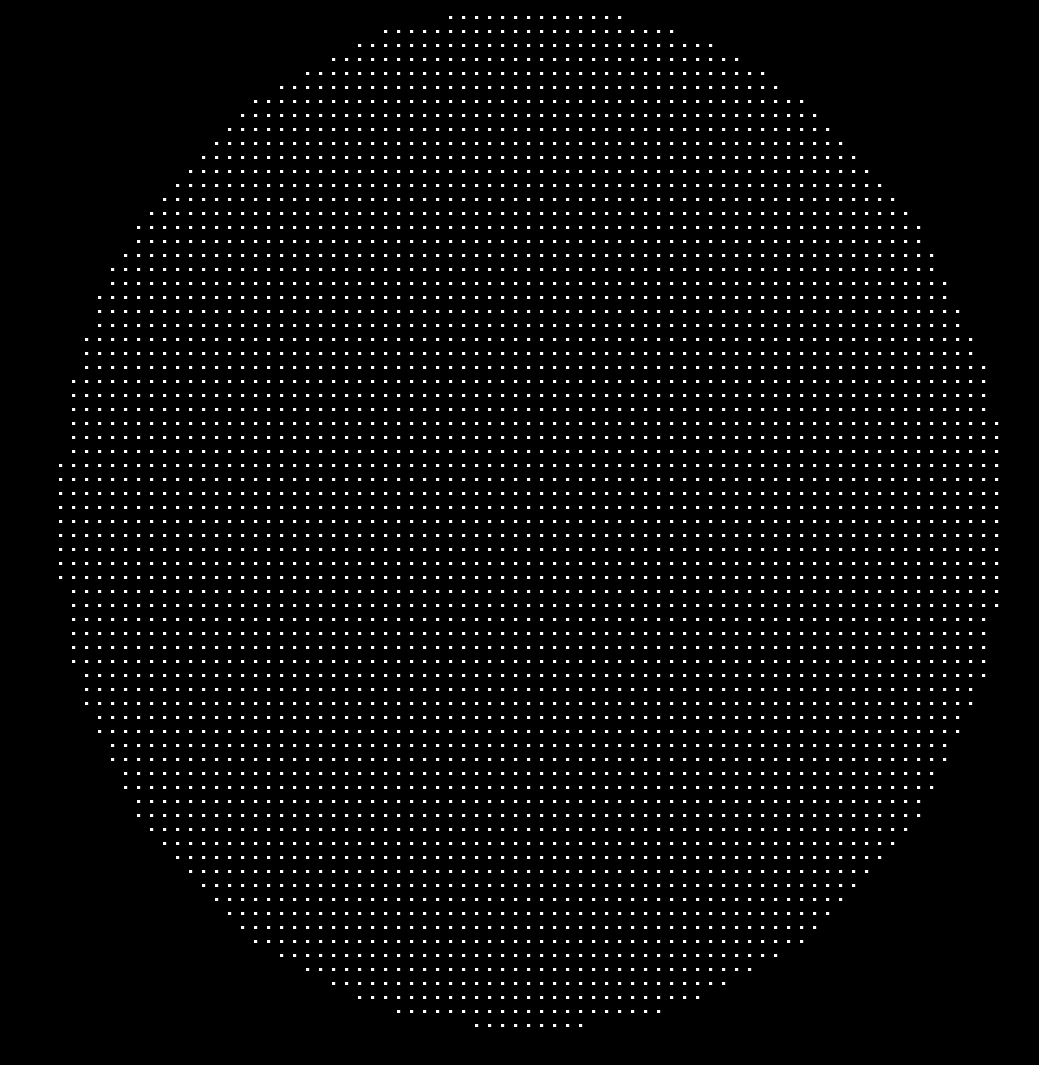
\includegraphics[scale=0.2]{images/test3.png}
    \caption{Источник света находится в точке с координатами (0, 0, 0)}
    \label{fig:test3}
\end{figure}

На рисунке \ref{fig:test4} источник света находится в точке с координатами (0, 0, -10), то есть перед сферой. Сфера освещена корректно.

\begin{figure}[H]
    \centering
    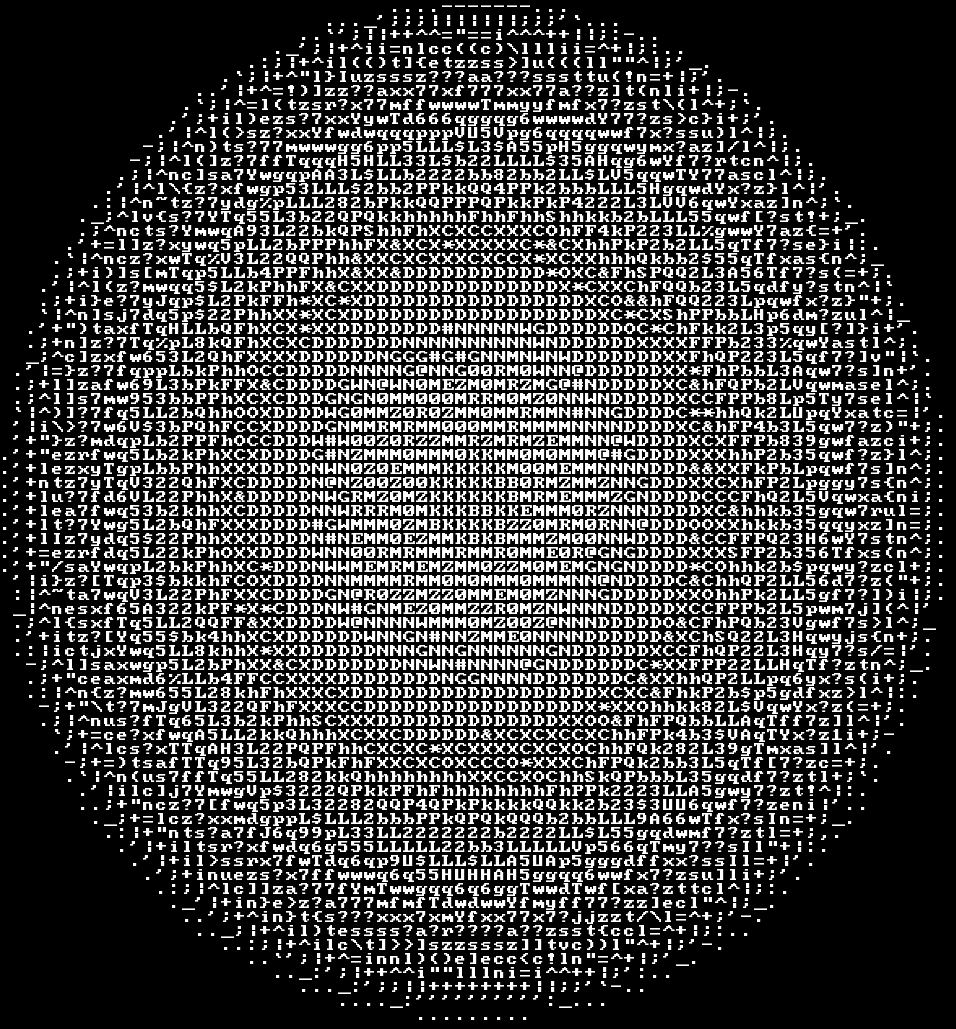
\includegraphics[scale=0.2]{images/test4.png}
    \caption{Источник света находится в точке с координатами (0, 0, -10)}
    \label{fig:test4}
\end{figure}

На рисунке \ref{fig:test5} источник света находится в точке с координатами (0, 0, 10), то есть за сферой. Как и ожидалось, освещённую часть сферы не видно.

\begin{figure}[H]
    \centering
    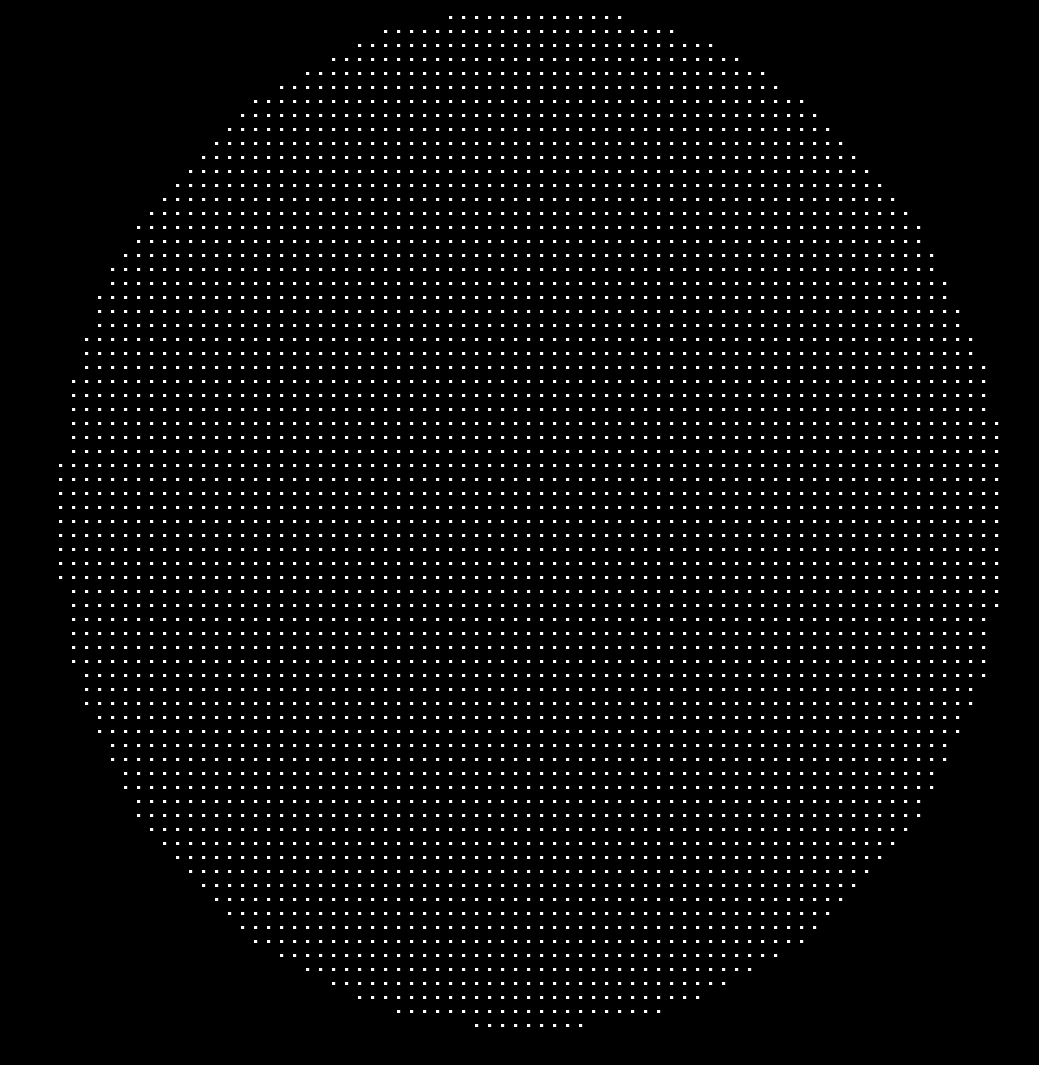
\includegraphics[scale=0.2]{images/test3.png}
    \caption{Источник света находится в точке с координатами (0, 0, 10)}
    \label{fig:test5}
\end{figure}

\section{Выводы из технологической части}

Было реализовано программное обеспечение для построения трёхмерного изображения объёмных объектов, а также проведено его функциональное тестирование. 

\clearpage
